% Options for packages loaded elsewhere
\PassOptionsToPackage{unicode}{hyperref}
\PassOptionsToPackage{hyphens}{url}
%
\documentclass[
]{article}
\usepackage{amsmath,amssymb}
\usepackage{iftex}
\ifPDFTeX
  \usepackage[T1]{fontenc}
  \usepackage[utf8]{inputenc}
  \usepackage{textcomp} % provide euro and other symbols
\else % if luatex or xetex
  \usepackage{unicode-math} % this also loads fontspec
  \defaultfontfeatures{Scale=MatchLowercase}
  \defaultfontfeatures[\rmfamily]{Ligatures=TeX,Scale=1}
\fi
\usepackage{lmodern}
\ifPDFTeX\else
  % xetex/luatex font selection
\fi
% Use upquote if available, for straight quotes in verbatim environments
\IfFileExists{upquote.sty}{\usepackage{upquote}}{}
\IfFileExists{microtype.sty}{% use microtype if available
  \usepackage[]{microtype}
  \UseMicrotypeSet[protrusion]{basicmath} % disable protrusion for tt fonts
}{}
\makeatletter
\@ifundefined{KOMAClassName}{% if non-KOMA class
  \IfFileExists{parskip.sty}{%
    \usepackage{parskip}
  }{% else
    \setlength{\parindent}{0pt}
    \setlength{\parskip}{6pt plus 2pt minus 1pt}}
}{% if KOMA class
  \KOMAoptions{parskip=half}}
\makeatother
\usepackage{xcolor}
\usepackage[margin=1in]{geometry}
\usepackage{color}
\usepackage{fancyvrb}
\newcommand{\VerbBar}{|}
\newcommand{\VERB}{\Verb[commandchars=\\\{\}]}
\DefineVerbatimEnvironment{Highlighting}{Verbatim}{commandchars=\\\{\}}
% Add ',fontsize=\small' for more characters per line
\usepackage{framed}
\definecolor{shadecolor}{RGB}{248,248,248}
\newenvironment{Shaded}{\begin{snugshade}}{\end{snugshade}}
\newcommand{\AlertTok}[1]{\textcolor[rgb]{0.94,0.16,0.16}{#1}}
\newcommand{\AnnotationTok}[1]{\textcolor[rgb]{0.56,0.35,0.01}{\textbf{\textit{#1}}}}
\newcommand{\AttributeTok}[1]{\textcolor[rgb]{0.13,0.29,0.53}{#1}}
\newcommand{\BaseNTok}[1]{\textcolor[rgb]{0.00,0.00,0.81}{#1}}
\newcommand{\BuiltInTok}[1]{#1}
\newcommand{\CharTok}[1]{\textcolor[rgb]{0.31,0.60,0.02}{#1}}
\newcommand{\CommentTok}[1]{\textcolor[rgb]{0.56,0.35,0.01}{\textit{#1}}}
\newcommand{\CommentVarTok}[1]{\textcolor[rgb]{0.56,0.35,0.01}{\textbf{\textit{#1}}}}
\newcommand{\ConstantTok}[1]{\textcolor[rgb]{0.56,0.35,0.01}{#1}}
\newcommand{\ControlFlowTok}[1]{\textcolor[rgb]{0.13,0.29,0.53}{\textbf{#1}}}
\newcommand{\DataTypeTok}[1]{\textcolor[rgb]{0.13,0.29,0.53}{#1}}
\newcommand{\DecValTok}[1]{\textcolor[rgb]{0.00,0.00,0.81}{#1}}
\newcommand{\DocumentationTok}[1]{\textcolor[rgb]{0.56,0.35,0.01}{\textbf{\textit{#1}}}}
\newcommand{\ErrorTok}[1]{\textcolor[rgb]{0.64,0.00,0.00}{\textbf{#1}}}
\newcommand{\ExtensionTok}[1]{#1}
\newcommand{\FloatTok}[1]{\textcolor[rgb]{0.00,0.00,0.81}{#1}}
\newcommand{\FunctionTok}[1]{\textcolor[rgb]{0.13,0.29,0.53}{\textbf{#1}}}
\newcommand{\ImportTok}[1]{#1}
\newcommand{\InformationTok}[1]{\textcolor[rgb]{0.56,0.35,0.01}{\textbf{\textit{#1}}}}
\newcommand{\KeywordTok}[1]{\textcolor[rgb]{0.13,0.29,0.53}{\textbf{#1}}}
\newcommand{\NormalTok}[1]{#1}
\newcommand{\OperatorTok}[1]{\textcolor[rgb]{0.81,0.36,0.00}{\textbf{#1}}}
\newcommand{\OtherTok}[1]{\textcolor[rgb]{0.56,0.35,0.01}{#1}}
\newcommand{\PreprocessorTok}[1]{\textcolor[rgb]{0.56,0.35,0.01}{\textit{#1}}}
\newcommand{\RegionMarkerTok}[1]{#1}
\newcommand{\SpecialCharTok}[1]{\textcolor[rgb]{0.81,0.36,0.00}{\textbf{#1}}}
\newcommand{\SpecialStringTok}[1]{\textcolor[rgb]{0.31,0.60,0.02}{#1}}
\newcommand{\StringTok}[1]{\textcolor[rgb]{0.31,0.60,0.02}{#1}}
\newcommand{\VariableTok}[1]{\textcolor[rgb]{0.00,0.00,0.00}{#1}}
\newcommand{\VerbatimStringTok}[1]{\textcolor[rgb]{0.31,0.60,0.02}{#1}}
\newcommand{\WarningTok}[1]{\textcolor[rgb]{0.56,0.35,0.01}{\textbf{\textit{#1}}}}
\usepackage{graphicx}
\makeatletter
\def\maxwidth{\ifdim\Gin@nat@width>\linewidth\linewidth\else\Gin@nat@width\fi}
\def\maxheight{\ifdim\Gin@nat@height>\textheight\textheight\else\Gin@nat@height\fi}
\makeatother
% Scale images if necessary, so that they will not overflow the page
% margins by default, and it is still possible to overwrite the defaults
% using explicit options in \includegraphics[width, height, ...]{}
\setkeys{Gin}{width=\maxwidth,height=\maxheight,keepaspectratio}
% Set default figure placement to htbp
\makeatletter
\def\fps@figure{htbp}
\makeatother
\setlength{\emergencystretch}{3em} % prevent overfull lines
\providecommand{\tightlist}{%
  \setlength{\itemsep}{0pt}\setlength{\parskip}{0pt}}
\setcounter{secnumdepth}{-\maxdimen} % remove section numbering
\ifLuaTeX
  \usepackage{selnolig}  % disable illegal ligatures
\fi
\usepackage{bookmark}
\IfFileExists{xurl.sty}{\usepackage{xurl}}{} % add URL line breaks if available
\urlstyle{same}
\hypersetup{
  pdftitle={Color Analysis Code},
  pdfauthor={Sara Shapiro},
  hidelinks,
  pdfcreator={LaTeX via pandoc}}

\title{Color Analysis Code}
\author{Sara Shapiro}
\date{2025-01-03}

\begin{document}
\maketitle

\subsection{Script for lobster color data
analysis}\label{script-for-lobster-color-data-analysis}

load the following packages: library(ggplot2) library(ggfortify)
library(tidyverse) library(ggpubr) require(patchwork) library(gginnards)
library(reshape) library(Ternary) library(ggrain) library(ggsignif)
library(dplyr) library(ggtern)

Note: In the following examples, I only included dummy data for one
temperature.

\section{Set the working directory and import the .csv
file}\label{set-the-working-directory-and-import-the-.csv-file}

\begin{Shaded}
\begin{Highlighting}[]
\FunctionTok{setwd}\NormalTok{(}\StringTok{"C:/Users/sks/Documents/Tepolt Lab/2024\_PL\_lab\_images/github"}\NormalTok{)}
\NormalTok{data }\OtherTok{\textless{}{-}} \FunctionTok{read.csv}\NormalTok{(}\StringTok{"dummy\_data.csv"}\NormalTok{)}
\end{Highlighting}
\end{Shaded}

\section{Set up data frames for each
ROI}\label{set-up-data-frames-for-each-roi}

\begin{Shaded}
\begin{Highlighting}[]
\NormalTok{CH\_R }\OtherTok{\textless{}{-}} \FunctionTok{c}\NormalTok{(data}\SpecialCharTok{$}\NormalTok{CH\_R)}
\NormalTok{CH\_G }\OtherTok{\textless{}{-}} \FunctionTok{c}\NormalTok{(data}\SpecialCharTok{$}\NormalTok{CH\_G)}
\NormalTok{CH\_B }\OtherTok{\textless{}{-}} \FunctionTok{c}\NormalTok{(data}\SpecialCharTok{$}\NormalTok{CH\_B)}
\NormalTok{lob }\OtherTok{\textless{}{-}} \FunctionTok{c}\NormalTok{(data}\SpecialCharTok{$}\NormalTok{Lobster)}
\NormalTok{date }\OtherTok{\textless{}{-}} \FunctionTok{c}\NormalTok{(data}\SpecialCharTok{$}\NormalTok{Date)}
\NormalTok{uv }\OtherTok{\textless{}{-}} \FunctionTok{c}\NormalTok{(data}\SpecialCharTok{$}\NormalTok{UV\_Treatment)}
\NormalTok{temp }\OtherTok{\textless{}{-}} \FunctionTok{c}\NormalTok{(data}\SpecialCharTok{$}\NormalTok{Temp)}
\NormalTok{df\_CH }\OtherTok{\textless{}{-}} \FunctionTok{data.frame}\NormalTok{(lob,temp,date,uv,CH\_R,CH\_G,CH\_B)}

\NormalTok{CTM\_R }\OtherTok{\textless{}{-}} \FunctionTok{c}\NormalTok{(data}\SpecialCharTok{$}\NormalTok{CTM\_R)}
\NormalTok{CTM\_G }\OtherTok{\textless{}{-}} \FunctionTok{c}\NormalTok{(data}\SpecialCharTok{$}\NormalTok{CTM\_G)}
\NormalTok{CTM\_B }\OtherTok{\textless{}{-}} \FunctionTok{c}\NormalTok{(data}\SpecialCharTok{$}\NormalTok{CTM\_B)}
\NormalTok{df\_CTM }\OtherTok{\textless{}{-}} \FunctionTok{data.frame}\NormalTok{(lob,temp,date,uv,CTM\_R,CTM\_G,CTM\_B)}

\NormalTok{CTE\_R }\OtherTok{\textless{}{-}} \FunctionTok{c}\NormalTok{(data}\SpecialCharTok{$}\NormalTok{CTE\_R)}
\NormalTok{CTE\_G }\OtherTok{\textless{}{-}} \FunctionTok{c}\NormalTok{(data}\SpecialCharTok{$}\NormalTok{CTE\_G)}
\NormalTok{CTE\_B }\OtherTok{\textless{}{-}} \FunctionTok{c}\NormalTok{(data}\SpecialCharTok{$}\NormalTok{CTE\_B)}
\NormalTok{df\_CTE }\OtherTok{\textless{}{-}} \FunctionTok{data.frame}\NormalTok{(lob,temp,date,uv,CTE\_R,CTE\_G,CTE\_B)}

\NormalTok{AS2\_R }\OtherTok{\textless{}{-}} \FunctionTok{c}\NormalTok{(data}\SpecialCharTok{$}\NormalTok{AS}\FloatTok{.2}\NormalTok{\_R)}
\NormalTok{AS2\_G }\OtherTok{\textless{}{-}} \FunctionTok{c}\NormalTok{(data}\SpecialCharTok{$}\NormalTok{AS}\FloatTok{.2}\NormalTok{\_G)}
\NormalTok{AS2\_B }\OtherTok{\textless{}{-}} \FunctionTok{c}\NormalTok{(data}\SpecialCharTok{$}\NormalTok{AS}\FloatTok{.2}\NormalTok{\_B)}
\NormalTok{df\_AS2 }\OtherTok{\textless{}{-}} \FunctionTok{data.frame}\NormalTok{(lob,temp,date,uv,AS2\_R,AS2\_G,AS2\_B)}

\NormalTok{AS5\_R }\OtherTok{\textless{}{-}} \FunctionTok{c}\NormalTok{(data}\SpecialCharTok{$}\NormalTok{AS}\FloatTok{.5}\NormalTok{\_R)}
\NormalTok{AS5\_G }\OtherTok{\textless{}{-}} \FunctionTok{c}\NormalTok{(data}\SpecialCharTok{$}\NormalTok{AS}\FloatTok{.5}\NormalTok{\_G)}
\NormalTok{AS5\_B }\OtherTok{\textless{}{-}} \FunctionTok{c}\NormalTok{(data}\SpecialCharTok{$}\NormalTok{AS}\FloatTok{.5}\NormalTok{\_B)}
\NormalTok{df\_AS5 }\OtherTok{\textless{}{-}} \FunctionTok{data.frame}\NormalTok{(lob,temp,date,uv,AS5\_R,AS5\_G,AS5\_B)}
\end{Highlighting}
\end{Shaded}

\section{Color Grid Example}\label{color-grid-example}

\begin{Shaded}
\begin{Highlighting}[]
\NormalTok{uv.labs }\OtherTok{\textless{}{-}} \FunctionTok{c}\NormalTok{(}\StringTok{"UV Treatment"}\NormalTok{, }\StringTok{"Non{-}UV Treatment"}\NormalTok{) }\CommentTok{\# formatting to re{-}label facet titles}
\FunctionTok{names}\NormalTok{(uv.labs) }\OtherTok{\textless{}{-}} \FunctionTok{c}\NormalTok{(}\StringTok{"UV"}\NormalTok{, }\StringTok{"X"}\NormalTok{) }\CommentTok{\# connecting the old labels with the new labels}

\NormalTok{ch18\_cg }\OtherTok{\textless{}{-}} \FunctionTok{ggplot}\NormalTok{(df\_CH, }\FunctionTok{aes}\NormalTok{(}\AttributeTok{x =}\NormalTok{ date, }\AttributeTok{y =}\NormalTok{ lob)) }\SpecialCharTok{+}
  \FunctionTok{geom\_raster}\NormalTok{(}\FunctionTok{aes}\NormalTok{(}\AttributeTok{fill =} \FunctionTok{rgb}\NormalTok{(CH\_R, CH\_G, CH\_B, }\AttributeTok{maxColorValue =} \DecValTok{255}\NormalTok{))) }\SpecialCharTok{+}
  \FunctionTok{scale\_fill\_identity}\NormalTok{() }\SpecialCharTok{+}
  \FunctionTok{facet\_wrap}\NormalTok{(. }\SpecialCharTok{\textasciitilde{}}\NormalTok{ uv, }\AttributeTok{scales =} \StringTok{"free\_y"}\NormalTok{, }\AttributeTok{labeller =} \FunctionTok{labeller}\NormalTok{(}\AttributeTok{uv =}\NormalTok{ uv.labs)) }\SpecialCharTok{+}
  \FunctionTok{labs}\NormalTok{(}\AttributeTok{title =} \StringTok{"Chelae 18C"}\NormalTok{, }\AttributeTok{x =} \StringTok{"Date"}\NormalTok{, }\AttributeTok{y =} \StringTok{"Lobster"}\NormalTok{)}

\NormalTok{ch18\_cg}
\end{Highlighting}
\end{Shaded}

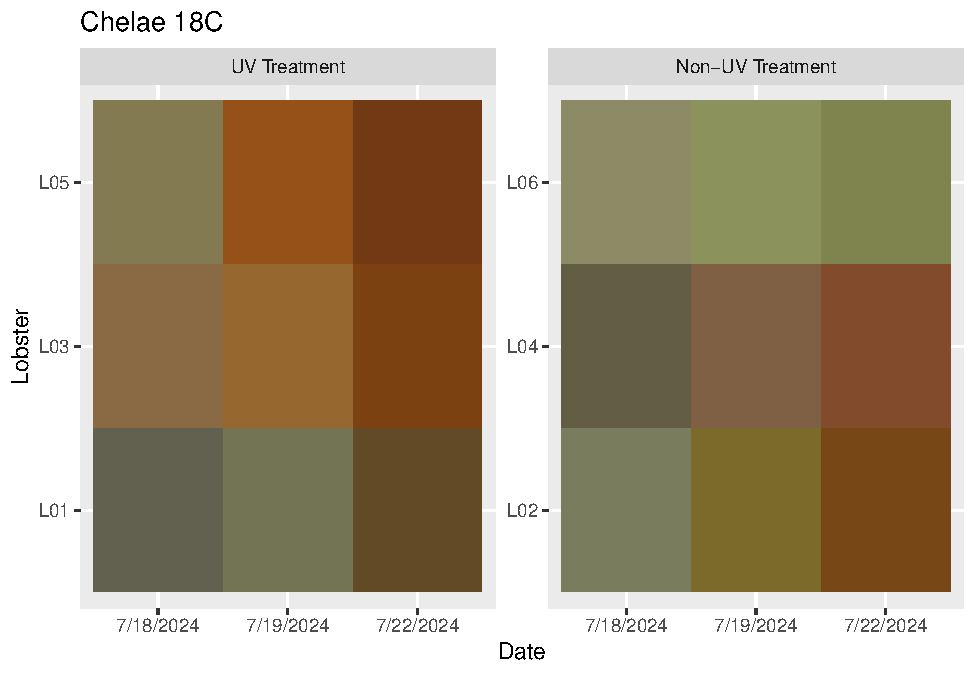
\includegraphics{color_analysis_pdf_files/figure-latex/Chelae_(CH)_Color Grid-1.pdf}

\section{Ternary Plot using ggtern
Example}\label{ternary-plot-using-ggtern-example}

Note: You can ignore the Warning message that states ``Ignoring unknown
aesthetics: z'', it doesn't impact the graph result

\begin{Shaded}
\begin{Highlighting}[]
\CommentTok{\# Create the base color spectrum that will color the background of the Ternary plot}
\NormalTok{all.colors }\OtherTok{\textless{}{-}} \FunctionTok{expand.grid}\NormalTok{(}\AttributeTok{R =} \DecValTok{0}\SpecialCharTok{:}\DecValTok{100}\NormalTok{, }\AttributeTok{G =} \DecValTok{0}\SpecialCharTok{:}\DecValTok{100}\NormalTok{, }\AttributeTok{B =} \DecValTok{0}\SpecialCharTok{:}\DecValTok{100}\NormalTok{)}
\NormalTok{all.colors }\OtherTok{\textless{}{-}}\NormalTok{ all.colors[}\FunctionTok{rowSums}\NormalTok{(all.colors) }\SpecialCharTok{==} \DecValTok{100}\NormalTok{, ]}
\NormalTok{all.colors }\OtherTok{\textless{}{-}}\NormalTok{ all.colors }\SpecialCharTok{/} \DecValTok{100}
\NormalTok{all.colors}\SpecialCharTok{$}\NormalTok{hex }\OtherTok{\textless{}{-}} \FunctionTok{with}\NormalTok{(all.colors, }\FunctionTok{rgb}\NormalTok{(R, G, B))}

\CommentTok{\# Create Ternary Plot}
\NormalTok{ch\_tern\_d1 }\OtherTok{\textless{}{-}} \FunctionTok{ggtern}\NormalTok{(all.colors, }\FunctionTok{aes}\NormalTok{(}\AttributeTok{x =}\NormalTok{ B, }\AttributeTok{y =}\NormalTok{ R, }\AttributeTok{z =}\NormalTok{ G)) }\SpecialCharTok{+} \CommentTok{\# this plots the background}
  \FunctionTok{geom\_point}\NormalTok{(}\FunctionTok{aes}\NormalTok{(}\AttributeTok{color =}\NormalTok{ hex), }\AttributeTok{size =} \DecValTok{3}\NormalTok{, }\AttributeTok{shape =} \DecValTok{17}\NormalTok{) }\SpecialCharTok{+} \CommentTok{\# this needs to reference all.colors in order for the background to properly fill}
  \FunctionTok{geom\_label}\NormalTok{(}\AttributeTok{data =}\NormalTok{ df\_CH, }\AttributeTok{inherit.aes =} \ConstantTok{FALSE}\NormalTok{, }\CommentTok{\# this is where you plot your data points}
    \AttributeTok{mapping =} \FunctionTok{aes}\NormalTok{(}\AttributeTok{x =}\NormalTok{ CH\_B, }\AttributeTok{y =}\NormalTok{ CH\_R, }\AttributeTok{z =}\NormalTok{ CH\_G, }\AttributeTok{label =}\NormalTok{ uv, }\AttributeTok{fill =}\NormalTok{ uv),}
    \AttributeTok{size =} \DecValTok{2}\NormalTok{, }\AttributeTok{alpha =} \FloatTok{0.7}\NormalTok{) }\SpecialCharTok{+}
  \FunctionTok{scale\_fill\_manual}\NormalTok{(}\AttributeTok{values=}\FunctionTok{c}\NormalTok{(}\StringTok{"white"}\NormalTok{, }\StringTok{"black"}\NormalTok{)) }\SpecialCharTok{+}
  \FunctionTok{facet\_grid}\NormalTok{(. }\SpecialCharTok{\textasciitilde{}}\NormalTok{ date) }\SpecialCharTok{+} \CommentTok{\# you could delete the facet if you want to create one graph for each date (you would just need to create a new data set for each date and change the geom\_label accordingly)}
  \FunctionTok{scale\_color\_identity}\NormalTok{() }\SpecialCharTok{+}
  \FunctionTok{scale\_L\_continuous}\NormalTok{(}\AttributeTok{breaks =} \FunctionTok{seq}\NormalTok{(}\DecValTok{0}\NormalTok{, }\DecValTok{1}\NormalTok{, }\FloatTok{0.1}\NormalTok{), }\AttributeTok{labels =} \FunctionTok{seq}\NormalTok{(}\DecValTok{0}\NormalTok{, }\DecValTok{1}\NormalTok{, }\FloatTok{0.1}\NormalTok{)) }\SpecialCharTok{+}
  \FunctionTok{scale\_T\_continuous}\NormalTok{(}\AttributeTok{breaks =} \FunctionTok{seq}\NormalTok{(}\DecValTok{0}\NormalTok{, }\DecValTok{1}\NormalTok{, }\FloatTok{0.1}\NormalTok{), }\AttributeTok{labels =} \FunctionTok{seq}\NormalTok{(}\DecValTok{0}\NormalTok{, }\DecValTok{1}\NormalTok{, }\FloatTok{0.1}\NormalTok{)) }\SpecialCharTok{+}
  \FunctionTok{scale\_R\_continuous}\NormalTok{(}\AttributeTok{breaks =} \FunctionTok{seq}\NormalTok{(}\DecValTok{0}\NormalTok{, }\DecValTok{1}\NormalTok{, }\FloatTok{0.1}\NormalTok{), }\AttributeTok{labels =} \FunctionTok{seq}\NormalTok{(}\DecValTok{0}\NormalTok{, }\DecValTok{1}\NormalTok{, }\FloatTok{0.1}\NormalTok{)) }\SpecialCharTok{+}
  \FunctionTok{theme\_rgbw}\NormalTok{(}\DecValTok{14}\NormalTok{) }\SpecialCharTok{+} 
  \FunctionTok{ggtitle}\NormalTok{(}\StringTok{"Chelae 18C Day 1"}\NormalTok{)}
\end{Highlighting}
\end{Shaded}

\begin{verbatim}
## Warning in geom_label(data = df_CH, inherit.aes = FALSE, mapping = aes(x =
## CH_B, : Ignoring unknown aesthetics: z
\end{verbatim}

\begin{Shaded}
\begin{Highlighting}[]
\NormalTok{ch\_tern\_d1}
\end{Highlighting}
\end{Shaded}

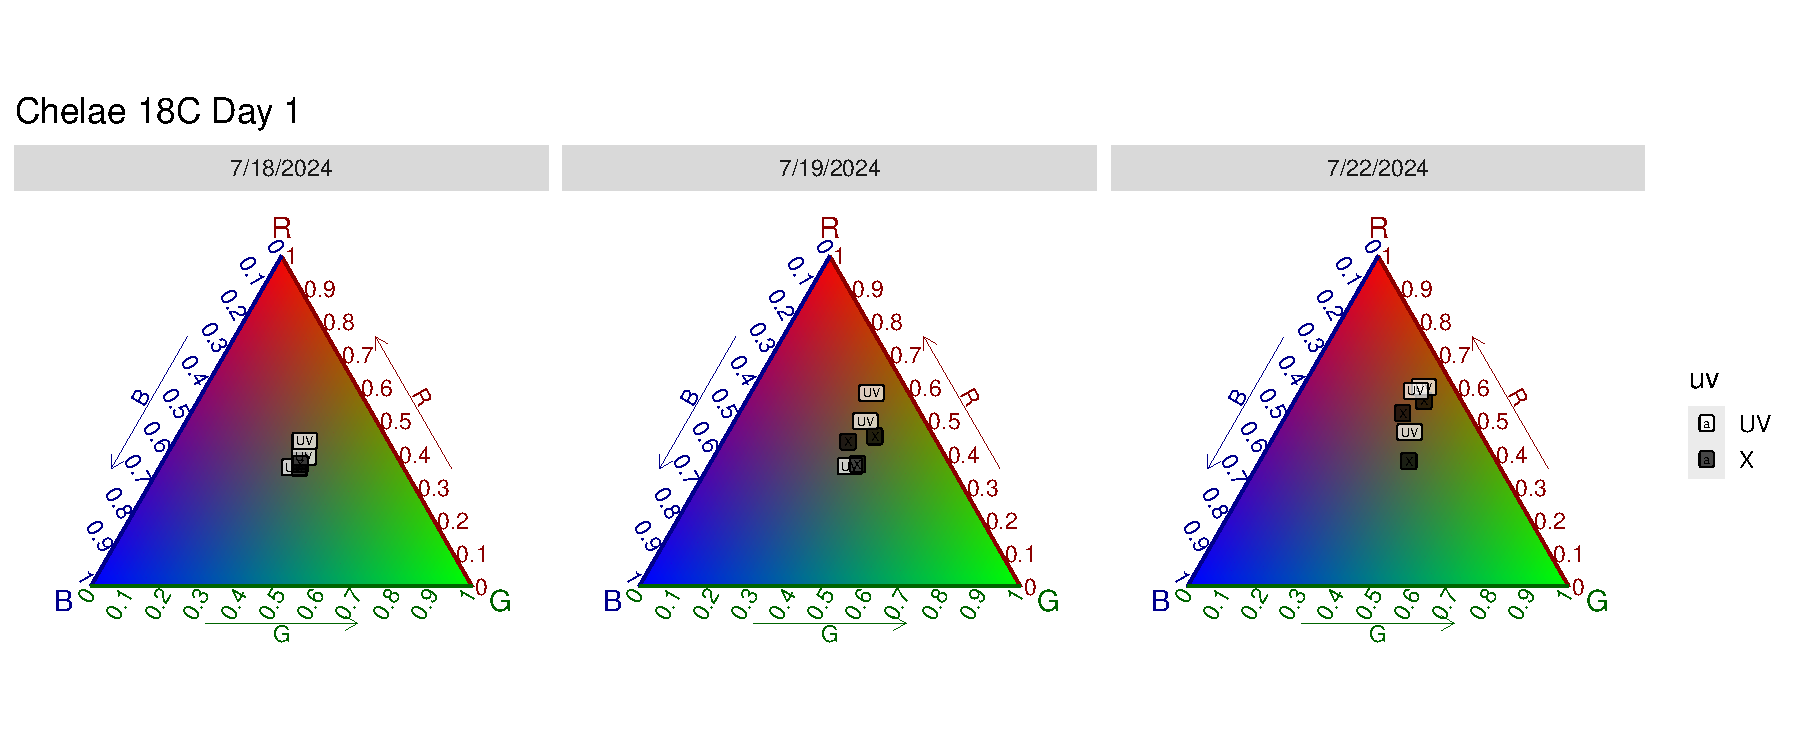
\includegraphics{color_analysis_pdf_files/figure-latex/ggtern Ternary Plot-1.pdf}

\section{Ternary Plot Example using Ternary
Package}\label{ternary-plot-example-using-ternary-package}

Note: You can add as many Ternary plots to one full graphing area at a
time, just adjust the graphing space mfrow parameters to accommodate all
plots. I haven't found a way to assign a figure data name to the plot,
so you have to manually save it in the Plots viewer (I find zooming in
helps with the dimensions).

\begin{Shaded}
\begin{Highlighting}[]
\NormalTok{ch18\_df }\OtherTok{\textless{}{-}}\NormalTok{ df\_CH }\SpecialCharTok{\%\textgreater{}\%} \CommentTok{\# creates a new column with the red, green, and blue values together}
\NormalTok{  rowwise }\SpecialCharTok{\%\textgreater{}\%}
  \FunctionTok{mutate}\NormalTok{(}\AttributeTok{ch =} \FunctionTok{list}\NormalTok{(}\FunctionTok{c}\NormalTok{(CH\_R,CH\_G,CH\_B))) }\SpecialCharTok{\%\textgreater{}\%}
\NormalTok{  ungroup}

\CommentTok{\# Create data sets for each day, separated by UV treatment}
\NormalTok{ch\_d1 }\OtherTok{\textless{}{-}} \FunctionTok{filter}\NormalTok{(ch18\_df, date }\SpecialCharTok{==} \StringTok{"7/18/2024"} \SpecialCharTok{\&}\NormalTok{ uv }\SpecialCharTok{==} \StringTok{"X"}\NormalTok{)}
\NormalTok{ch\_d1\_UV }\OtherTok{\textless{}{-}} \FunctionTok{filter}\NormalTok{(ch18\_df, date }\SpecialCharTok{==} \StringTok{"7/18/2024"} \SpecialCharTok{\&}\NormalTok{ uv }\SpecialCharTok{==} \StringTok{"UV"}\NormalTok{)}
\NormalTok{ch\_d2 }\OtherTok{\textless{}{-}} \FunctionTok{filter}\NormalTok{(ch18\_df, date }\SpecialCharTok{==} \StringTok{"7/19/2024"} \SpecialCharTok{\&}\NormalTok{ uv }\SpecialCharTok{==} \StringTok{"X"}\NormalTok{)}
\NormalTok{ch\_d2\_UV }\OtherTok{\textless{}{-}} \FunctionTok{filter}\NormalTok{(ch18\_df, date }\SpecialCharTok{==} \StringTok{"7/19/2024"} \SpecialCharTok{\&}\NormalTok{ uv }\SpecialCharTok{==} \StringTok{"UV"}\NormalTok{)}
\NormalTok{ch\_d5 }\OtherTok{\textless{}{-}} \FunctionTok{filter}\NormalTok{(ch18\_df, date }\SpecialCharTok{==} \StringTok{"7/22/2024"} \SpecialCharTok{\&}\NormalTok{ uv }\SpecialCharTok{==} \StringTok{"X"}\NormalTok{)}
\NormalTok{ch\_d5\_UV }\OtherTok{\textless{}{-}} \FunctionTok{filter}\NormalTok{(ch18\_df, date }\SpecialCharTok{==} \StringTok{"7/22/2024"} \SpecialCharTok{\&}\NormalTok{ uv }\SpecialCharTok{==} \StringTok{"UV"}\NormalTok{)}

\CommentTok{\# Create graphing space for Ternary Plots}
\FunctionTok{par}\NormalTok{(}\AttributeTok{mfrow =} \FunctionTok{c}\NormalTok{(}\DecValTok{1}\NormalTok{,}\DecValTok{3}\NormalTok{), }\AttributeTok{mar =} \FunctionTok{rep}\NormalTok{(}\FloatTok{0.3}\NormalTok{, }\DecValTok{4}\NormalTok{)) }\CommentTok{\# for mfrow = c(,), the first number is rows and second is columns; this sets up the space to plot the ternary plots}

\CommentTok{\# Make Day 1 Initial Ternary Plot}
\FunctionTok{TernaryPlot}\NormalTok{(}\AttributeTok{alab =} \StringTok{"Redder \textbackslash{}u2192"}\NormalTok{, }\AttributeTok{blab =} \StringTok{"Greener \textbackslash{}u2192"}\NormalTok{, }\AttributeTok{clab =} \StringTok{"\textbackslash{}u2190 Bluer"}\NormalTok{,}
            \AttributeTok{lab.col =} \FunctionTok{c}\NormalTok{(}\StringTok{"red"}\NormalTok{, }\StringTok{"darkgreen"}\NormalTok{, }\StringTok{"blue"}\NormalTok{),}
            \AttributeTok{main =} \StringTok{"CH {-} Day 1"}\NormalTok{, }\CommentTok{\# Title}
            \AttributeTok{point =} \StringTok{"up"}\NormalTok{, }\AttributeTok{lab.cex =} \DecValTok{1}\NormalTok{, }\AttributeTok{grid.minor.lines =} \DecValTok{0}\NormalTok{,}
            \AttributeTok{grid.lty =} \StringTok{"solid"}\NormalTok{, }\AttributeTok{col =} \FunctionTok{rgb}\NormalTok{(}\FloatTok{0.9}\NormalTok{, }\FloatTok{0.9}\NormalTok{, }\FloatTok{0.9}\NormalTok{), }\AttributeTok{grid.col =} \StringTok{"white"}\NormalTok{, }
            \AttributeTok{axis.col =} \FunctionTok{rgb}\NormalTok{(}\FloatTok{0.6}\NormalTok{, }\FloatTok{0.6}\NormalTok{, }\FloatTok{0.6}\NormalTok{), }\AttributeTok{ticks.col =} \FunctionTok{rgb}\NormalTok{(}\FloatTok{0.6}\NormalTok{, }\FloatTok{0.6}\NormalTok{, }\FloatTok{0.6}\NormalTok{),}
            \AttributeTok{axis.rotate =} \ConstantTok{FALSE}\NormalTok{,}
            \AttributeTok{padding =} \FloatTok{0.08}\NormalTok{,}
            \AttributeTok{axis.labels =} \FunctionTok{seq}\NormalTok{(}\DecValTok{0}\NormalTok{, }\DecValTok{10}\NormalTok{, }\AttributeTok{by =} \DecValTok{1}\NormalTok{),}
            \AttributeTok{xlim=}\ConstantTok{NULL}\NormalTok{,}
            \AttributeTok{isometric=}\ConstantTok{TRUE}\NormalTok{,}
\NormalTok{            )}

\CommentTok{\# Color the background}
\NormalTok{cols }\OtherTok{\textless{}{-}} \FunctionTok{TernaryPointValues}\NormalTok{(rgb)}
\FunctionTok{ColourTernary}\NormalTok{(cols, }\AttributeTok{spectrum =} \ConstantTok{NULL}\NormalTok{)}

\CommentTok{\# Add data points }
\NormalTok{ch\_d1\_18\_points }\OtherTok{\textless{}{-}}\NormalTok{ ch\_d1}\SpecialCharTok{$}\NormalTok{ch}
\FunctionTok{AddToTernary}\NormalTok{(points, ch\_d1\_18\_points, }\AttributeTok{pch =} \DecValTok{1}\NormalTok{, }\AttributeTok{cex =} \FloatTok{1.5}\NormalTok{, }\AttributeTok{col =} \FunctionTok{c}\NormalTok{(}\StringTok{"black"}\NormalTok{) , }\CommentTok{\#can change point type and color}
             \AttributeTok{bg =} \FunctionTok{vapply}\NormalTok{(ch\_d1\_18\_points, }
                         \ControlFlowTok{function}\NormalTok{ (x) }\FunctionTok{rgb}\NormalTok{(x[}\DecValTok{1}\NormalTok{], x[}\DecValTok{2}\NormalTok{], x[}\DecValTok{3}\NormalTok{], }\DecValTok{128}\NormalTok{,}
                                          \AttributeTok{maxColorValue =} \DecValTok{255}\NormalTok{),}
                         \FunctionTok{character}\NormalTok{(}\DecValTok{1}\NormalTok{))}
\NormalTok{)}

\NormalTok{ch\_d1\_18\_UV\_points }\OtherTok{\textless{}{-}}\NormalTok{ ch\_d1\_UV}\SpecialCharTok{$}\NormalTok{ch}
\FunctionTok{AddToTernary}\NormalTok{(points, ch\_d1\_18\_UV\_points, }\AttributeTok{pch =} \DecValTok{1}\NormalTok{, }\AttributeTok{cex =} \FloatTok{1.5}\NormalTok{, }\AttributeTok{col =} \FunctionTok{c}\NormalTok{(}\StringTok{"white"}\NormalTok{) , }
             \AttributeTok{bg =} \FunctionTok{vapply}\NormalTok{(ch\_d1\_18\_UV\_points, }
                         \ControlFlowTok{function}\NormalTok{ (x) }\FunctionTok{rgb}\NormalTok{(x[}\DecValTok{1}\NormalTok{], x[}\DecValTok{2}\NormalTok{], x[}\DecValTok{3}\NormalTok{], }\DecValTok{128}\NormalTok{,}
                                          \AttributeTok{maxColorValue =} \DecValTok{255}\NormalTok{),}
                         \FunctionTok{character}\NormalTok{(}\DecValTok{1}\NormalTok{))}
\NormalTok{)}

\CommentTok{\# Make Day 2 Initial Ternary Plot}
\FunctionTok{TernaryPlot}\NormalTok{(}\AttributeTok{alab =} \StringTok{"Redder \textbackslash{}u2192"}\NormalTok{, }\AttributeTok{blab =} \StringTok{"Greener \textbackslash{}u2192"}\NormalTok{, }\AttributeTok{clab =} \StringTok{"\textbackslash{}u2190 Bluer"}\NormalTok{,}
            \AttributeTok{lab.col =} \FunctionTok{c}\NormalTok{(}\StringTok{"red"}\NormalTok{, }\StringTok{"darkgreen"}\NormalTok{, }\StringTok{"blue"}\NormalTok{),}
            \AttributeTok{main =} \StringTok{"CH {-} Day 2"}\NormalTok{, }\CommentTok{\# Title}
            \AttributeTok{point =} \StringTok{"up"}\NormalTok{, }\AttributeTok{lab.cex =} \DecValTok{1}\NormalTok{, }\AttributeTok{grid.minor.lines =} \DecValTok{0}\NormalTok{,}
            \AttributeTok{grid.lty =} \StringTok{"solid"}\NormalTok{, }\AttributeTok{col =} \FunctionTok{rgb}\NormalTok{(}\FloatTok{0.9}\NormalTok{, }\FloatTok{0.9}\NormalTok{, }\FloatTok{0.9}\NormalTok{), }\AttributeTok{grid.col =} \StringTok{"white"}\NormalTok{, }
            \AttributeTok{axis.col =} \FunctionTok{rgb}\NormalTok{(}\FloatTok{0.6}\NormalTok{, }\FloatTok{0.6}\NormalTok{, }\FloatTok{0.6}\NormalTok{), }\AttributeTok{ticks.col =} \FunctionTok{rgb}\NormalTok{(}\FloatTok{0.6}\NormalTok{, }\FloatTok{0.6}\NormalTok{, }\FloatTok{0.6}\NormalTok{),}
            \AttributeTok{axis.rotate =} \ConstantTok{FALSE}\NormalTok{,}
            \AttributeTok{padding =} \FloatTok{0.08}\NormalTok{,}
            \AttributeTok{axis.labels =} \FunctionTok{seq}\NormalTok{(}\DecValTok{0}\NormalTok{, }\DecValTok{10}\NormalTok{, }\AttributeTok{by =} \DecValTok{1}\NormalTok{),}
            \AttributeTok{xlim=}\ConstantTok{NULL}\NormalTok{,}
            \AttributeTok{isometric=}\ConstantTok{TRUE}\NormalTok{,}
\NormalTok{            )}

\CommentTok{\# Color the background}
\NormalTok{cols }\OtherTok{\textless{}{-}} \FunctionTok{TernaryPointValues}\NormalTok{(rgb)}
\FunctionTok{ColourTernary}\NormalTok{(cols, }\AttributeTok{spectrum =} \ConstantTok{NULL}\NormalTok{)}

\CommentTok{\# Add data points}
\NormalTok{ch\_d2\_18\_points }\OtherTok{\textless{}{-}}\NormalTok{ ch\_d2}\SpecialCharTok{$}\NormalTok{ch}
\FunctionTok{AddToTernary}\NormalTok{(points, ch\_d2\_18\_points, }\AttributeTok{pch =} \DecValTok{1}\NormalTok{, }\AttributeTok{cex =} \FloatTok{1.5}\NormalTok{, }\AttributeTok{col =} \FunctionTok{c}\NormalTok{(}\StringTok{"black"}\NormalTok{) , }
             \AttributeTok{bg =} \FunctionTok{vapply}\NormalTok{(ch\_d2\_18\_points, }
                         \ControlFlowTok{function}\NormalTok{ (x) }\FunctionTok{rgb}\NormalTok{(x[}\DecValTok{1}\NormalTok{], x[}\DecValTok{2}\NormalTok{], x[}\DecValTok{3}\NormalTok{], }\DecValTok{128}\NormalTok{,}
                                          \AttributeTok{maxColorValue =} \DecValTok{255}\NormalTok{),}
                         \FunctionTok{character}\NormalTok{(}\DecValTok{1}\NormalTok{))}
\NormalTok{)}

\NormalTok{ch\_d2\_18\_UV\_points }\OtherTok{\textless{}{-}}\NormalTok{ ch\_d2\_UV}\SpecialCharTok{$}\NormalTok{ch}
\FunctionTok{AddToTernary}\NormalTok{(points, ch\_d2\_18\_UV\_points, }\AttributeTok{pch =} \DecValTok{1}\NormalTok{, }\AttributeTok{cex =} \FloatTok{1.5}\NormalTok{, }\AttributeTok{col =} \FunctionTok{c}\NormalTok{(}\StringTok{"white"}\NormalTok{) , }
             \AttributeTok{bg =} \FunctionTok{vapply}\NormalTok{(ch\_d2\_18\_UV\_points, }
                         \ControlFlowTok{function}\NormalTok{ (x) }\FunctionTok{rgb}\NormalTok{(x[}\DecValTok{1}\NormalTok{], x[}\DecValTok{2}\NormalTok{], x[}\DecValTok{3}\NormalTok{], }\DecValTok{128}\NormalTok{,}
                                          \AttributeTok{maxColorValue =} \DecValTok{255}\NormalTok{),}
                         \FunctionTok{character}\NormalTok{(}\DecValTok{1}\NormalTok{))}
\NormalTok{)}

\CommentTok{\# Make Day 2 Initial Ternary Plot}
\FunctionTok{TernaryPlot}\NormalTok{(}\AttributeTok{alab =} \StringTok{"Redder \textbackslash{}u2192"}\NormalTok{, }\AttributeTok{blab =} \StringTok{"Greener \textbackslash{}u2192"}\NormalTok{, }\AttributeTok{clab =} \StringTok{"\textbackslash{}u2190 Bluer"}\NormalTok{,}
            \AttributeTok{lab.col =} \FunctionTok{c}\NormalTok{(}\StringTok{"red"}\NormalTok{, }\StringTok{"darkgreen"}\NormalTok{, }\StringTok{"blue"}\NormalTok{),}
            \AttributeTok{main =} \StringTok{"CH {-} Day 5"}\NormalTok{, }\CommentTok{\# Title}
            \AttributeTok{point =} \StringTok{"up"}\NormalTok{, }\AttributeTok{lab.cex =} \DecValTok{1}\NormalTok{, }\AttributeTok{grid.minor.lines =} \DecValTok{0}\NormalTok{,}
            \AttributeTok{grid.lty =} \StringTok{"solid"}\NormalTok{, }\AttributeTok{col =} \FunctionTok{rgb}\NormalTok{(}\FloatTok{0.9}\NormalTok{, }\FloatTok{0.9}\NormalTok{, }\FloatTok{0.9}\NormalTok{), }\AttributeTok{grid.col =} \StringTok{"white"}\NormalTok{, }
            \AttributeTok{axis.col =} \FunctionTok{rgb}\NormalTok{(}\FloatTok{0.6}\NormalTok{, }\FloatTok{0.6}\NormalTok{, }\FloatTok{0.6}\NormalTok{), }\AttributeTok{ticks.col =} \FunctionTok{rgb}\NormalTok{(}\FloatTok{0.6}\NormalTok{, }\FloatTok{0.6}\NormalTok{, }\FloatTok{0.6}\NormalTok{),}
            \AttributeTok{axis.rotate =} \ConstantTok{FALSE}\NormalTok{,}
            \AttributeTok{padding =} \FloatTok{0.08}\NormalTok{,}
            \AttributeTok{axis.labels =} \FunctionTok{seq}\NormalTok{(}\DecValTok{0}\NormalTok{, }\DecValTok{10}\NormalTok{, }\AttributeTok{by =} \DecValTok{1}\NormalTok{),}
            \AttributeTok{xlim=}\ConstantTok{NULL}\NormalTok{,}
            \AttributeTok{isometric=}\ConstantTok{TRUE}\NormalTok{,}
\NormalTok{            )}

\CommentTok{\# Color the background}
\NormalTok{cols }\OtherTok{\textless{}{-}} \FunctionTok{TernaryPointValues}\NormalTok{(rgb)}
\FunctionTok{ColourTernary}\NormalTok{(cols, }\AttributeTok{spectrum =} \ConstantTok{NULL}\NormalTok{)}

\CommentTok{\# Add data points}
\NormalTok{ch\_d5\_18\_points }\OtherTok{\textless{}{-}}\NormalTok{ ch\_d5}\SpecialCharTok{$}\NormalTok{ch}
\FunctionTok{AddToTernary}\NormalTok{(points, ch\_d5\_18\_points, }\AttributeTok{pch =} \DecValTok{1}\NormalTok{, }\AttributeTok{cex =} \FloatTok{1.5}\NormalTok{, }\AttributeTok{col =} \FunctionTok{c}\NormalTok{(}\StringTok{"black"}\NormalTok{) , }
             \AttributeTok{bg =} \FunctionTok{vapply}\NormalTok{(ch\_d5\_18\_points, }
                         \ControlFlowTok{function}\NormalTok{ (x) }\FunctionTok{rgb}\NormalTok{(x[}\DecValTok{1}\NormalTok{], x[}\DecValTok{2}\NormalTok{], x[}\DecValTok{3}\NormalTok{], }\DecValTok{128}\NormalTok{,}
                                          \AttributeTok{maxColorValue =} \DecValTok{255}\NormalTok{),}
                         \FunctionTok{character}\NormalTok{(}\DecValTok{1}\NormalTok{))}
\NormalTok{)}

\NormalTok{ch\_d5\_18\_UV\_points }\OtherTok{\textless{}{-}}\NormalTok{ ch\_d5\_UV}\SpecialCharTok{$}\NormalTok{ch}
\FunctionTok{AddToTernary}\NormalTok{(points, ch\_d5\_18\_UV\_points, }\AttributeTok{pch =} \DecValTok{1}\NormalTok{, }\AttributeTok{cex =} \FloatTok{1.5}\NormalTok{, }\AttributeTok{col =} \FunctionTok{c}\NormalTok{(}\StringTok{"white"}\NormalTok{) , }
             \AttributeTok{bg =} \FunctionTok{vapply}\NormalTok{(ch\_d5\_18\_UV\_points, }
                         \ControlFlowTok{function}\NormalTok{ (x) }\FunctionTok{rgb}\NormalTok{(x[}\DecValTok{1}\NormalTok{], x[}\DecValTok{2}\NormalTok{], x[}\DecValTok{3}\NormalTok{], }\DecValTok{128}\NormalTok{,}
                                          \AttributeTok{maxColorValue =} \DecValTok{255}\NormalTok{),}
                         \FunctionTok{character}\NormalTok{(}\DecValTok{1}\NormalTok{))}
\NormalTok{)}
\end{Highlighting}
\end{Shaded}

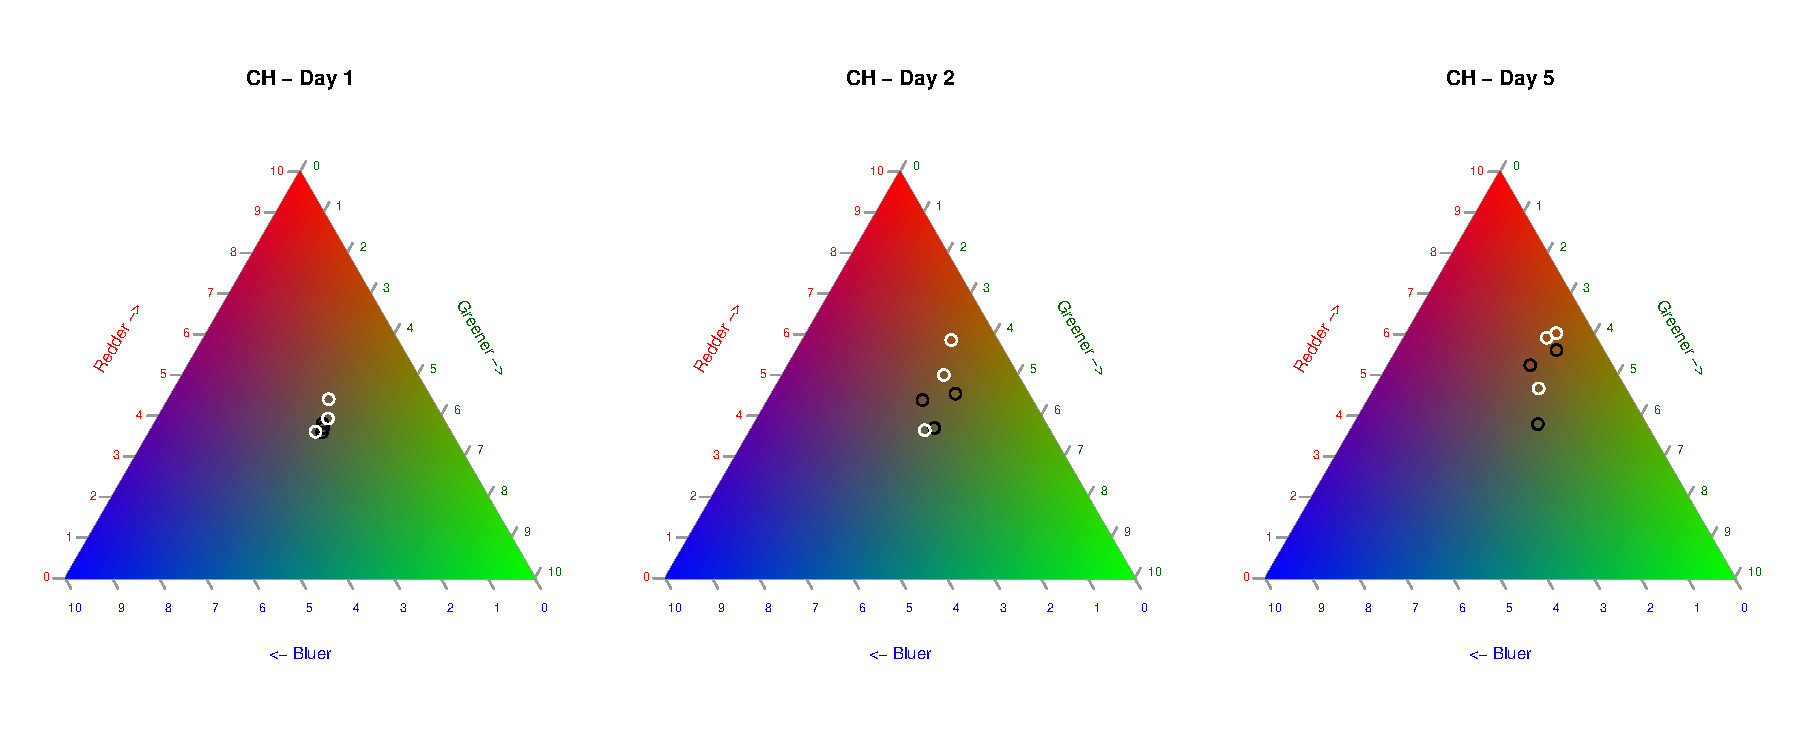
\includegraphics{color_analysis_pdf_files/figure-latex/Ternary w/ Ternary Package-1.pdf}

\section{Boxplots Example}\label{boxplots-example}

Graphs the Red, Green, and Blue values for each region across time to
see if there's any significant change in any of the colors between
treatments over time. Interpretation of results: if colors decrease,
then overall pigment is getting darker; if colors increase, then overall
pigment is getting lighter; increase and/or no change in one color while
other colors decrease would result in pigment change towards the
increased and/or no change color (ex. Red inc/same, Green \& Blue dec
-\textgreater{} overall pigment would be redder).

Note: Significance in these plots is comparing treatments over time, not
within each treatment over time. Roughly speaking, it's comparing the
slopes of the geom\_smooth function for each treatment.

\begin{Shaded}
\begin{Highlighting}[]
\CommentTok{\# Create data frames for each color}
\NormalTok{df\_R }\OtherTok{\textless{}{-}} \FunctionTok{data.frame}\NormalTok{(lob,date,temp,uv,CH\_R,CTM\_R,CTE\_R,AS2\_R,AS5\_R)}
\NormalTok{df\_R}\SpecialCharTok{$}\NormalTok{uv }\OtherTok{\textless{}{-}} \FunctionTok{factor}\NormalTok{(df\_R}\SpecialCharTok{$}\NormalTok{uv, }\AttributeTok{levels =} \FunctionTok{c}\NormalTok{(}\StringTok{"X"}\NormalTok{,}\StringTok{"UV"}\NormalTok{))}
\NormalTok{df\_G }\OtherTok{\textless{}{-}} \FunctionTok{data.frame}\NormalTok{(lob,date,temp,uv,CH\_G,CTM\_G,CTE\_G,AS2\_G,AS5\_G)}
\NormalTok{df\_G}\SpecialCharTok{$}\NormalTok{uv }\OtherTok{\textless{}{-}} \FunctionTok{factor}\NormalTok{(df\_G}\SpecialCharTok{$}\NormalTok{uv, }\AttributeTok{levels =} \FunctionTok{c}\NormalTok{(}\StringTok{"X"}\NormalTok{,}\StringTok{"UV"}\NormalTok{))}
\NormalTok{df\_B }\OtherTok{\textless{}{-}} \FunctionTok{data.frame}\NormalTok{(lob,date,temp,uv,CH\_B,CTM\_B,CTE\_B,AS2\_B,AS5\_B)}
\NormalTok{df\_B}\SpecialCharTok{$}\NormalTok{uv }\OtherTok{\textless{}{-}} \FunctionTok{factor}\NormalTok{(df\_B}\SpecialCharTok{$}\NormalTok{uv, }\AttributeTok{levels =} \FunctionTok{c}\NormalTok{(}\StringTok{"X"}\NormalTok{,}\StringTok{"UV"}\NormalTok{))}

\NormalTok{kw\_chR }\OtherTok{\textless{}{-}} \FunctionTok{kruskal.test}\NormalTok{(CH\_R }\SpecialCharTok{\textasciitilde{}}\NormalTok{ uv, }\AttributeTok{data =}\NormalTok{ df\_R) }\CommentTok{\# get Kruskal{-}Wallis value comparing color and UV treatment}
\NormalTok{pval\_kw\_chR }\OtherTok{\textless{}{-}}\NormalTok{ kw\_chR}\SpecialCharTok{$}\NormalTok{p.value }\CommentTok{\# create p value for Kruskal{-}Wallis test for plot}

\NormalTok{kw\_chG }\OtherTok{\textless{}{-}} \FunctionTok{kruskal.test}\NormalTok{(CH\_G }\SpecialCharTok{\textasciitilde{}}\NormalTok{ uv, }\AttributeTok{data =}\NormalTok{ df\_G)}
\NormalTok{pval\_kw\_chG }\OtherTok{\textless{}{-}}\NormalTok{ kw\_chG}\SpecialCharTok{$}\NormalTok{p.value}

\NormalTok{kw\_chB }\OtherTok{\textless{}{-}} \FunctionTok{kruskal.test}\NormalTok{(CH\_B }\SpecialCharTok{\textasciitilde{}}\NormalTok{ uv, }\AttributeTok{data =}\NormalTok{ df\_B)}
\NormalTok{pval\_kw\_chB }\OtherTok{\textless{}{-}}\NormalTok{ kw\_chB}\SpecialCharTok{$}\NormalTok{p.value}

\NormalTok{bp\_CH\_R }\OtherTok{\textless{}{-}} \FunctionTok{ggplot}\NormalTok{(df\_R,}\FunctionTok{aes}\NormalTok{(}\AttributeTok{x=}\FunctionTok{factor}\NormalTok{(date), }\AttributeTok{y=}\NormalTok{CH\_R, }\AttributeTok{color=}\NormalTok{uv, }\AttributeTok{fill=}\NormalTok{uv)) }\SpecialCharTok{+}
  \FunctionTok{geom\_boxplot}\NormalTok{(}\FunctionTok{aes}\NormalTok{(}\AttributeTok{fill =}\NormalTok{ uv), }\AttributeTok{alpha =} \FloatTok{0.50}\NormalTok{) }\SpecialCharTok{+} 
  \FunctionTok{scale\_fill\_manual}\NormalTok{(}\AttributeTok{values =} \FunctionTok{c}\NormalTok{(}\StringTok{"gray38"}\NormalTok{,}\StringTok{"white"}\NormalTok{)) }\SpecialCharTok{+} 
  \FunctionTok{labs}\NormalTok{(}\AttributeTok{y =} \StringTok{"CH\_R"}\NormalTok{, }\AttributeTok{x =} \StringTok{"Date"}\NormalTok{) }\SpecialCharTok{+} \FunctionTok{ggtitle}\NormalTok{(}\StringTok{"18C Chelae Red"}\NormalTok{) }\SpecialCharTok{+} 
  \FunctionTok{scale\_color\_manual}\NormalTok{(}\AttributeTok{values =} \FunctionTok{c}\NormalTok{(}\StringTok{"black"}\NormalTok{, }\StringTok{"black"}\NormalTok{)) }\SpecialCharTok{+} 
  \FunctionTok{theme}\NormalTok{(}\AttributeTok{legend.text=}\FunctionTok{element\_text}\NormalTok{(}\AttributeTok{size=}\DecValTok{12}\NormalTok{), }\AttributeTok{legend.key.size=}\FunctionTok{unit}\NormalTok{(}\DecValTok{2}\NormalTok{, }\StringTok{\textquotesingle{}cm\textquotesingle{}}\NormalTok{)) }\SpecialCharTok{+}
  \FunctionTok{theme}\NormalTok{(}\AttributeTok{axis.text.x =} \FunctionTok{element\_text}\NormalTok{(}\AttributeTok{angle=}\DecValTok{60}\NormalTok{, }\AttributeTok{hjust=}\DecValTok{1}\NormalTok{)) }\SpecialCharTok{+}
  \FunctionTok{theme}\NormalTok{(}\AttributeTok{text =} \FunctionTok{element\_text}\NormalTok{(}\AttributeTok{size =} \DecValTok{15}\NormalTok{), }\AttributeTok{plot.title =} \FunctionTok{element\_text}\NormalTok{(}\AttributeTok{color=}\StringTok{"firebrick"}\NormalTok{))}\SpecialCharTok{+}
  \FunctionTok{ylim}\NormalTok{(}\DecValTok{0}\NormalTok{,}\DecValTok{255}\NormalTok{) }\SpecialCharTok{+}
  \FunctionTok{geom\_smooth}\NormalTok{(}\FunctionTok{aes}\NormalTok{(}\AttributeTok{group=}\NormalTok{uv, }\AttributeTok{linetype =}\NormalTok{ uv), }\AttributeTok{linewidth =} \DecValTok{1}\NormalTok{, }\AttributeTok{method =} \StringTok{"glm"}\NormalTok{, }\AttributeTok{se =} \ConstantTok{FALSE}\NormalTok{)}\SpecialCharTok{+}
  \FunctionTok{annotate}\NormalTok{(}\StringTok{"text"}\NormalTok{, }\AttributeTok{x =} \ConstantTok{Inf}\NormalTok{, }\AttributeTok{y =} \ConstantTok{Inf}\NormalTok{, }
           \AttributeTok{label =} \FunctionTok{paste}\NormalTok{(}\StringTok{"p kw ="}\NormalTok{, }\FunctionTok{format.pval}\NormalTok{(pval\_kw\_chR, }\AttributeTok{digits =} \DecValTok{3}\NormalTok{)),}
           \AttributeTok{hjust =} \DecValTok{1}\NormalTok{, }\AttributeTok{vjust =} \DecValTok{1}\NormalTok{, }\AttributeTok{size =} \DecValTok{5}\NormalTok{)}

\NormalTok{bp\_CH\_G }\OtherTok{\textless{}{-}} \FunctionTok{ggplot}\NormalTok{(df\_G,}\FunctionTok{aes}\NormalTok{(}\AttributeTok{x=}\FunctionTok{factor}\NormalTok{(date), }\AttributeTok{y=}\NormalTok{CH\_G, }\AttributeTok{color=}\NormalTok{uv, }\AttributeTok{fill=}\NormalTok{uv)) }\SpecialCharTok{+}
  \FunctionTok{geom\_boxplot}\NormalTok{(}\FunctionTok{aes}\NormalTok{(}\AttributeTok{fill =}\NormalTok{ uv), }\AttributeTok{alpha =} \FloatTok{0.50}\NormalTok{) }\SpecialCharTok{+} 
  \FunctionTok{scale\_fill\_manual}\NormalTok{(}\AttributeTok{values =} \FunctionTok{c}\NormalTok{(}\StringTok{"gray38"}\NormalTok{,}\StringTok{"white"}\NormalTok{)) }\SpecialCharTok{+} 
  \FunctionTok{labs}\NormalTok{(}\AttributeTok{y =} \StringTok{"CH\_R"}\NormalTok{, }\AttributeTok{x =} \StringTok{"Date"}\NormalTok{) }\SpecialCharTok{+} \FunctionTok{ggtitle}\NormalTok{(}\StringTok{"18C Chelae Green"}\NormalTok{) }\SpecialCharTok{+} 
  \FunctionTok{scale\_color\_manual}\NormalTok{(}\AttributeTok{values =} \FunctionTok{c}\NormalTok{(}\StringTok{"black"}\NormalTok{, }\StringTok{"black"}\NormalTok{)) }\SpecialCharTok{+} 
  \FunctionTok{theme}\NormalTok{(}\AttributeTok{legend.text=}\FunctionTok{element\_text}\NormalTok{(}\AttributeTok{size=}\DecValTok{12}\NormalTok{), }\AttributeTok{legend.key.size=}\FunctionTok{unit}\NormalTok{(}\DecValTok{2}\NormalTok{, }\StringTok{\textquotesingle{}cm\textquotesingle{}}\NormalTok{)) }\SpecialCharTok{+}
  \FunctionTok{theme}\NormalTok{(}\AttributeTok{axis.text.x =} \FunctionTok{element\_text}\NormalTok{(}\AttributeTok{angle=}\DecValTok{60}\NormalTok{, }\AttributeTok{hjust=}\DecValTok{1}\NormalTok{)) }\SpecialCharTok{+}
  \FunctionTok{theme}\NormalTok{(}\AttributeTok{text =} \FunctionTok{element\_text}\NormalTok{(}\AttributeTok{size =} \DecValTok{15}\NormalTok{), }\AttributeTok{plot.title=} \FunctionTok{element\_text}\NormalTok{(}\AttributeTok{color=}\StringTok{"chartreuse4"}\NormalTok{))}\SpecialCharTok{+}
  \FunctionTok{ylim}\NormalTok{(}\DecValTok{0}\NormalTok{,}\DecValTok{255}\NormalTok{)}\SpecialCharTok{+}
  \FunctionTok{geom\_smooth}\NormalTok{(}\FunctionTok{aes}\NormalTok{(}\AttributeTok{group=}\NormalTok{uv, }\AttributeTok{linetype =}\NormalTok{ uv), }\AttributeTok{linewidth =} \DecValTok{1}\NormalTok{, }\AttributeTok{method =} \StringTok{"glm"}\NormalTok{, }\AttributeTok{se =} \ConstantTok{FALSE}\NormalTok{)}\SpecialCharTok{+}
  \FunctionTok{annotate}\NormalTok{(}\StringTok{"text"}\NormalTok{, }\AttributeTok{x =} \ConstantTok{Inf}\NormalTok{, }\AttributeTok{y =} \ConstantTok{Inf}\NormalTok{, }
           \AttributeTok{label =} \FunctionTok{paste}\NormalTok{(}\StringTok{"p kw ="}\NormalTok{, }\FunctionTok{format.pval}\NormalTok{(pval\_kw\_chG, }\AttributeTok{digits =} \DecValTok{3}\NormalTok{)),}
           \AttributeTok{hjust =} \DecValTok{1}\NormalTok{, }\AttributeTok{vjust =} \DecValTok{1}\NormalTok{, }\AttributeTok{size =} \DecValTok{5}\NormalTok{)}

\NormalTok{bp\_CH\_B }\OtherTok{\textless{}{-}} \FunctionTok{ggplot}\NormalTok{(df\_B,}\FunctionTok{aes}\NormalTok{(}\AttributeTok{x=}\FunctionTok{factor}\NormalTok{(date), }\AttributeTok{y=}\NormalTok{CH\_B, }\AttributeTok{color=}\NormalTok{uv, }\AttributeTok{fill=}\NormalTok{uv)) }\SpecialCharTok{+}
  \FunctionTok{geom\_boxplot}\NormalTok{(}\FunctionTok{aes}\NormalTok{(}\AttributeTok{fill =}\NormalTok{ uv), }\AttributeTok{alpha =} \FloatTok{0.50}\NormalTok{) }\SpecialCharTok{+} 
  \FunctionTok{scale\_fill\_manual}\NormalTok{(}\AttributeTok{values =} \FunctionTok{c}\NormalTok{(}\StringTok{"gray38"}\NormalTok{,}\StringTok{"white"}\NormalTok{)) }\SpecialCharTok{+} 
  \FunctionTok{labs}\NormalTok{(}\AttributeTok{y =} \StringTok{"CH\_R"}\NormalTok{, }\AttributeTok{x =} \StringTok{"Date"}\NormalTok{) }\SpecialCharTok{+} \FunctionTok{ggtitle}\NormalTok{(}\StringTok{"18C Chelae Blue"}\NormalTok{) }\SpecialCharTok{+} 
  \FunctionTok{scale\_color\_manual}\NormalTok{(}\AttributeTok{values =} \FunctionTok{c}\NormalTok{(}\StringTok{"black"}\NormalTok{, }\StringTok{"black"}\NormalTok{)) }\SpecialCharTok{+} 
  \FunctionTok{theme}\NormalTok{(}\AttributeTok{legend.text=}\FunctionTok{element\_text}\NormalTok{(}\AttributeTok{size=}\DecValTok{12}\NormalTok{), }\AttributeTok{legend.key.size=}\FunctionTok{unit}\NormalTok{(}\DecValTok{2}\NormalTok{, }\StringTok{\textquotesingle{}cm\textquotesingle{}}\NormalTok{)) }\SpecialCharTok{+}
  \FunctionTok{theme}\NormalTok{(}\AttributeTok{axis.text.x =} \FunctionTok{element\_text}\NormalTok{(}\AttributeTok{angle=}\DecValTok{60}\NormalTok{, }\AttributeTok{hjust=}\DecValTok{1}\NormalTok{)) }\SpecialCharTok{+}
  \FunctionTok{theme}\NormalTok{(}\AttributeTok{text =} \FunctionTok{element\_text}\NormalTok{(}\AttributeTok{size =} \DecValTok{15}\NormalTok{), }\AttributeTok{plot.title=} \FunctionTok{element\_text}\NormalTok{(}\AttributeTok{color=}\StringTok{"blue"}\NormalTok{))}\SpecialCharTok{+}
  \FunctionTok{ylim}\NormalTok{(}\DecValTok{0}\NormalTok{,}\DecValTok{255}\NormalTok{)}\SpecialCharTok{+}
  \FunctionTok{geom\_smooth}\NormalTok{(}\FunctionTok{aes}\NormalTok{(}\AttributeTok{group=}\NormalTok{uv, }\AttributeTok{linetype =}\NormalTok{ uv), }\AttributeTok{linewidth =} \DecValTok{1}\NormalTok{, }\AttributeTok{method =} \StringTok{"glm"}\NormalTok{, }\AttributeTok{se =} \ConstantTok{FALSE}\NormalTok{)}\SpecialCharTok{+}
  \FunctionTok{annotate}\NormalTok{(}\StringTok{"text"}\NormalTok{, }\AttributeTok{x =} \ConstantTok{Inf}\NormalTok{, }\AttributeTok{y =} \ConstantTok{Inf}\NormalTok{, }
           \AttributeTok{label =} \FunctionTok{paste}\NormalTok{(}\StringTok{"p kw ="}\NormalTok{, }\FunctionTok{format.pval}\NormalTok{(pval\_kw\_chB, }\AttributeTok{digits =} \DecValTok{3}\NormalTok{)),}
           \AttributeTok{hjust =} \DecValTok{1}\NormalTok{, }\AttributeTok{vjust =} \DecValTok{1}\NormalTok{, }\AttributeTok{size =} \DecValTok{5}\NormalTok{)}

\NormalTok{CH\_bp }\OtherTok{\textless{}{-}}\NormalTok{ ((bp\_CH\_R }\SpecialCharTok{+}\NormalTok{ bp\_CH\_G }\SpecialCharTok{+}\NormalTok{ bp\_CH\_B) }\SpecialCharTok{+} \FunctionTok{plot\_layout}\NormalTok{(}\AttributeTok{guides =} \StringTok{"collect"}\NormalTok{))}
\NormalTok{CH\_bp}
\end{Highlighting}
\end{Shaded}

\begin{verbatim}
## `geom_smooth()` using formula = 'y ~ x'
## `geom_smooth()` using formula = 'y ~ x'
## `geom_smooth()` using formula = 'y ~ x'
\end{verbatim}

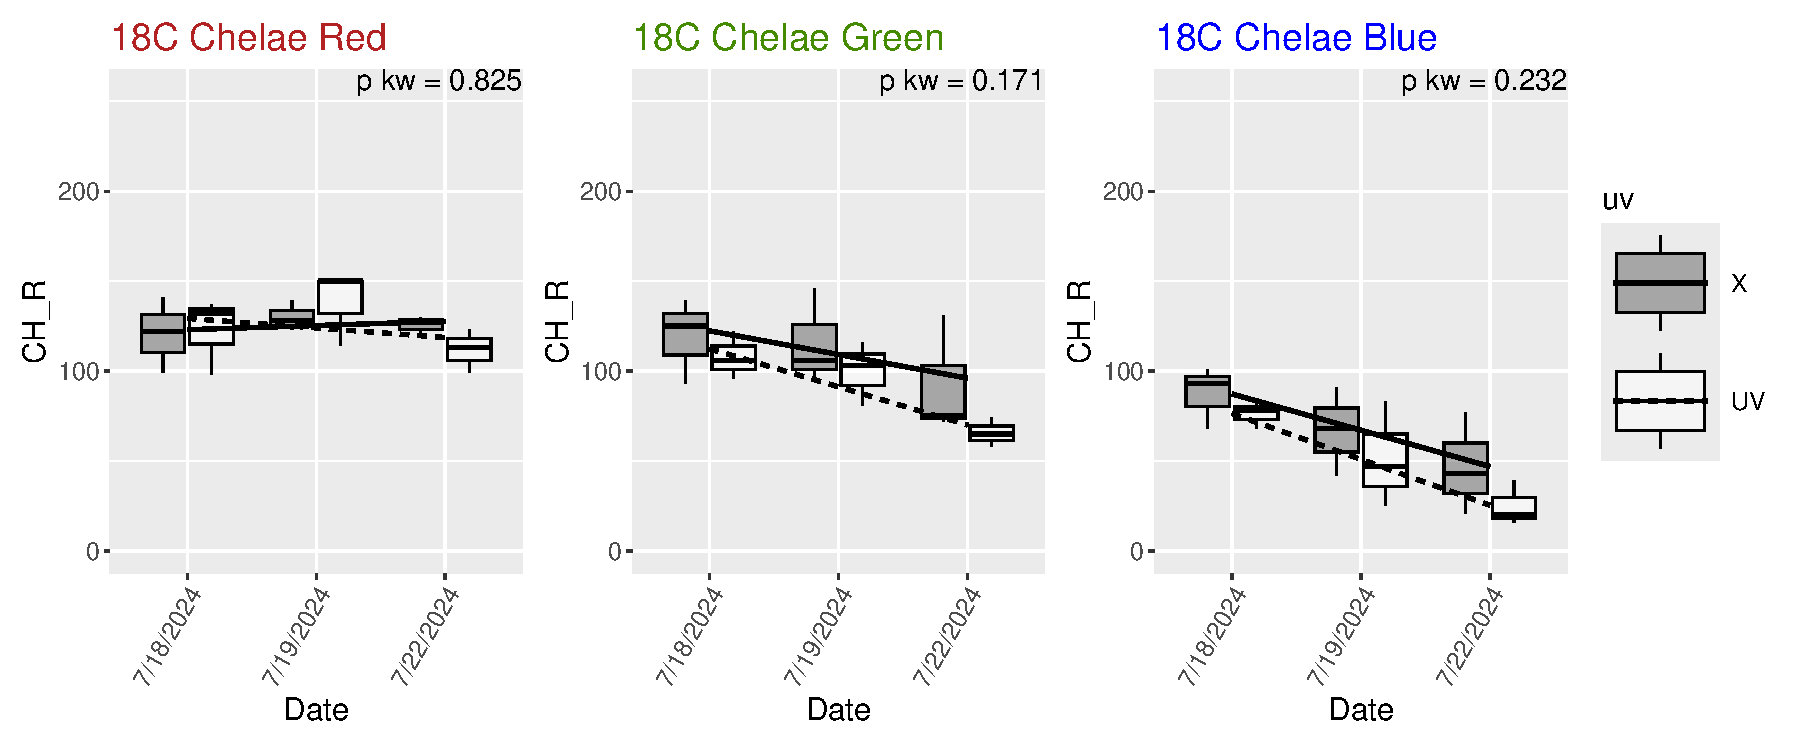
\includegraphics{color_analysis_pdf_files/figure-latex/Boxplots Example-1.pdf}

\section{Line Plots Example}\label{line-plots-example}

These line plots follow individuals over time and the significance is
the same as the boxplots.

\begin{Shaded}
\begin{Highlighting}[]
\CommentTok{\# Create the line plots (using the same Kruskal{-}Wallis P{-}value from above)}
\NormalTok{lp\_CH\_R }\OtherTok{\textless{}{-}} \FunctionTok{ggplot}\NormalTok{(df\_CH,}\FunctionTok{aes}\NormalTok{(date,CH\_R, }\AttributeTok{fill=}\NormalTok{uv, }\AttributeTok{color=}\NormalTok{uv, }\AttributeTok{group=}\NormalTok{lob)) }\SpecialCharTok{+}
  \FunctionTok{geom\_point}\NormalTok{(}\FunctionTok{aes}\NormalTok{(}\AttributeTok{fill=}\NormalTok{uv)) }\SpecialCharTok{+} \FunctionTok{geom\_line}\NormalTok{(}\FunctionTok{aes}\NormalTok{(}\AttributeTok{color=}\NormalTok{uv), }\AttributeTok{alpha=}\FloatTok{0.4}\NormalTok{) }\SpecialCharTok{+} 
  \FunctionTok{stat\_smooth}\NormalTok{(}\FunctionTok{aes}\NormalTok{(}\AttributeTok{group=}\NormalTok{uv), }\AttributeTok{linewidth =} \FloatTok{1.5}\NormalTok{, }\AttributeTok{method =} \StringTok{"glm"}\NormalTok{, }\AttributeTok{se =} \ConstantTok{FALSE}\NormalTok{) }\SpecialCharTok{+}
  \FunctionTok{stat\_summary}\NormalTok{(}\AttributeTok{fun =}\NormalTok{ mean, }\AttributeTok{geom =} \StringTok{"line"}\NormalTok{, }\FunctionTok{aes}\NormalTok{(}\AttributeTok{group =}\NormalTok{ uv, }\AttributeTok{color =}\NormalTok{ uv)) }\SpecialCharTok{+}
  \FunctionTok{theme\_classic}\NormalTok{() }\SpecialCharTok{+}
  \FunctionTok{theme}\NormalTok{(}\AttributeTok{axis.text.x =} \FunctionTok{element\_text}\NormalTok{(}\AttributeTok{angle=}\DecValTok{60}\NormalTok{, }\AttributeTok{hjust=}\DecValTok{1}\NormalTok{)) }\SpecialCharTok{+}
  \FunctionTok{scale\_fill\_manual}\NormalTok{(}\AttributeTok{values=}\FunctionTok{c}\NormalTok{(}\StringTok{"mediumorchid3"}\NormalTok{, }\StringTok{"deepskyblue3"}\NormalTok{)) }\SpecialCharTok{+}
  \FunctionTok{scale\_color\_manual}\NormalTok{(}\AttributeTok{values=}\FunctionTok{c}\NormalTok{(}\StringTok{"mediumorchid3"}\NormalTok{, }\StringTok{"deepskyblue3"}\NormalTok{)) }\SpecialCharTok{+}
  \FunctionTok{ggtitle}\NormalTok{(}\StringTok{"Red Chelae 18C Values"}\NormalTok{) }\SpecialCharTok{+} 
  \FunctionTok{theme}\NormalTok{(}\AttributeTok{plot.title =} \FunctionTok{element\_text}\NormalTok{(}\AttributeTok{color=}\StringTok{"firebrick"}\NormalTok{)) }\SpecialCharTok{+}
  \FunctionTok{ylim}\NormalTok{(}\DecValTok{0}\NormalTok{,}\DecValTok{255}\NormalTok{)}\SpecialCharTok{+}
  \FunctionTok{annotate}\NormalTok{(}\StringTok{"text"}\NormalTok{, }\AttributeTok{x =} \ConstantTok{Inf}\NormalTok{, }\AttributeTok{y =} \ConstantTok{Inf}\NormalTok{, }
           \AttributeTok{label =} \FunctionTok{paste}\NormalTok{(}\StringTok{"p kw ="}\NormalTok{, }\FunctionTok{format.pval}\NormalTok{(pval\_kw\_chR, }\AttributeTok{digits =} \DecValTok{3}\NormalTok{)),}
           \AttributeTok{hjust =} \DecValTok{1}\NormalTok{, }\AttributeTok{vjust =} \DecValTok{1}\NormalTok{, }\AttributeTok{size =} \DecValTok{5}\NormalTok{)}

\NormalTok{lp\_CH\_G }\OtherTok{\textless{}{-}} \FunctionTok{ggplot}\NormalTok{(df\_CH,}\FunctionTok{aes}\NormalTok{(date,CH\_G, }\AttributeTok{fill=}\NormalTok{uv, }\AttributeTok{color=}\NormalTok{uv, }\AttributeTok{group=}\NormalTok{lob)) }\SpecialCharTok{+}
  \FunctionTok{geom\_point}\NormalTok{(}\FunctionTok{aes}\NormalTok{(}\AttributeTok{fill=}\NormalTok{uv)) }\SpecialCharTok{+} \FunctionTok{geom\_line}\NormalTok{(}\FunctionTok{aes}\NormalTok{(}\AttributeTok{color=}\NormalTok{uv), }\AttributeTok{alpha=}\FloatTok{0.4}\NormalTok{) }\SpecialCharTok{+} 
  \FunctionTok{geom\_smooth}\NormalTok{(}\FunctionTok{aes}\NormalTok{(}\AttributeTok{group=}\NormalTok{uv), }\AttributeTok{linewidth =} \FloatTok{1.5}\NormalTok{, }\AttributeTok{method =} \StringTok{"glm"}\NormalTok{, }\AttributeTok{se =} \ConstantTok{FALSE}\NormalTok{) }\SpecialCharTok{+}
  \FunctionTok{stat\_summary}\NormalTok{(}\AttributeTok{fun =}\NormalTok{ mean, }\AttributeTok{geom =} \StringTok{"line"}\NormalTok{, }\FunctionTok{aes}\NormalTok{(}\AttributeTok{group =}\NormalTok{ uv, }\AttributeTok{color =}\NormalTok{ uv)) }\SpecialCharTok{+}
  \FunctionTok{theme\_classic}\NormalTok{() }\SpecialCharTok{+}
  \FunctionTok{theme}\NormalTok{(}\AttributeTok{axis.text.x =} \FunctionTok{element\_text}\NormalTok{(}\AttributeTok{angle=}\DecValTok{60}\NormalTok{, }\AttributeTok{hjust=}\DecValTok{1}\NormalTok{)) }\SpecialCharTok{+}
  \FunctionTok{scale\_fill\_manual}\NormalTok{(}\AttributeTok{values=}\FunctionTok{c}\NormalTok{(}\StringTok{"mediumorchid3"}\NormalTok{, }\StringTok{"deepskyblue3"}\NormalTok{)) }\SpecialCharTok{+}
  \FunctionTok{scale\_color\_manual}\NormalTok{(}\AttributeTok{values=}\FunctionTok{c}\NormalTok{(}\StringTok{"mediumorchid3"}\NormalTok{, }\StringTok{"deepskyblue3"}\NormalTok{)) }\SpecialCharTok{+}
  \FunctionTok{ggtitle}\NormalTok{(}\StringTok{"Green Chelae 18C Values"}\NormalTok{) }\SpecialCharTok{+} 
  \FunctionTok{theme}\NormalTok{(}\AttributeTok{plot.title =} \FunctionTok{element\_text}\NormalTok{(}\AttributeTok{color=}\StringTok{"chartreuse4"}\NormalTok{)) }\SpecialCharTok{+}
  \FunctionTok{ylim}\NormalTok{(}\DecValTok{0}\NormalTok{,}\DecValTok{255}\NormalTok{)}\SpecialCharTok{+}
  \FunctionTok{annotate}\NormalTok{(}\StringTok{"text"}\NormalTok{, }\AttributeTok{x =} \ConstantTok{Inf}\NormalTok{, }\AttributeTok{y =} \ConstantTok{Inf}\NormalTok{, }
           \AttributeTok{label =} \FunctionTok{paste}\NormalTok{(}\StringTok{"p kw ="}\NormalTok{, }\FunctionTok{format.pval}\NormalTok{(pval\_kw\_chG, }\AttributeTok{digits =} \DecValTok{3}\NormalTok{)),}
           \AttributeTok{hjust =} \DecValTok{1}\NormalTok{, }\AttributeTok{vjust =} \DecValTok{1}\NormalTok{, }\AttributeTok{size =} \DecValTok{5}\NormalTok{)}

\NormalTok{lp\_CH\_B }\OtherTok{\textless{}{-}} \FunctionTok{ggplot}\NormalTok{(df\_CH,}\FunctionTok{aes}\NormalTok{(date,CH\_B, }\AttributeTok{fill=}\NormalTok{uv, }\AttributeTok{color=}\NormalTok{uv, }\AttributeTok{group=}\NormalTok{lob)) }\SpecialCharTok{+}
  \FunctionTok{geom\_point}\NormalTok{(}\FunctionTok{aes}\NormalTok{(}\AttributeTok{fill=}\NormalTok{uv)) }\SpecialCharTok{+} \FunctionTok{geom\_line}\NormalTok{(}\FunctionTok{aes}\NormalTok{(}\AttributeTok{color=}\NormalTok{uv), }\AttributeTok{alpha=}\FloatTok{0.4}\NormalTok{) }\SpecialCharTok{+} 
  \FunctionTok{geom\_smooth}\NormalTok{(}\FunctionTok{aes}\NormalTok{(}\AttributeTok{group=}\NormalTok{uv), }\AttributeTok{linewidth =} \FloatTok{1.5}\NormalTok{, }\AttributeTok{method =} \StringTok{"glm"}\NormalTok{, }\AttributeTok{se =} \ConstantTok{FALSE}\NormalTok{) }\SpecialCharTok{+}
  \FunctionTok{stat\_summary}\NormalTok{(}\AttributeTok{fun =}\NormalTok{ mean, }\AttributeTok{geom =} \StringTok{"line"}\NormalTok{, }\FunctionTok{aes}\NormalTok{(}\AttributeTok{group =}\NormalTok{ uv, }\AttributeTok{color =}\NormalTok{ uv)) }\SpecialCharTok{+}
  \FunctionTok{theme\_classic}\NormalTok{() }\SpecialCharTok{+}
  \FunctionTok{theme}\NormalTok{(}\AttributeTok{axis.text.x =} \FunctionTok{element\_text}\NormalTok{(}\AttributeTok{angle=}\DecValTok{60}\NormalTok{, }\AttributeTok{hjust=}\DecValTok{1}\NormalTok{)) }\SpecialCharTok{+}
  \FunctionTok{scale\_fill\_manual}\NormalTok{(}\AttributeTok{values=}\FunctionTok{c}\NormalTok{(}\StringTok{"mediumorchid3"}\NormalTok{, }\StringTok{"deepskyblue3"}\NormalTok{)) }\SpecialCharTok{+}
  \FunctionTok{scale\_color\_manual}\NormalTok{(}\AttributeTok{values=}\FunctionTok{c}\NormalTok{(}\StringTok{"mediumorchid3"}\NormalTok{, }\StringTok{"deepskyblue3"}\NormalTok{)) }\SpecialCharTok{+}
  \FunctionTok{ggtitle}\NormalTok{(}\StringTok{"Blue Chelae 18C Values"}\NormalTok{) }\SpecialCharTok{+} 
  \FunctionTok{theme}\NormalTok{(}\AttributeTok{plot.title =} \FunctionTok{element\_text}\NormalTok{(}\AttributeTok{color=}\StringTok{"blue"}\NormalTok{)) }\SpecialCharTok{+}
  \FunctionTok{ylim}\NormalTok{(}\DecValTok{0}\NormalTok{,}\DecValTok{255}\NormalTok{)}\SpecialCharTok{+}
  \FunctionTok{annotate}\NormalTok{(}\StringTok{"text"}\NormalTok{, }\AttributeTok{x =} \ConstantTok{Inf}\NormalTok{, }\AttributeTok{y =} \ConstantTok{Inf}\NormalTok{, }
           \AttributeTok{label =} \FunctionTok{paste}\NormalTok{(}\StringTok{"p kw ="}\NormalTok{, }\FunctionTok{format.pval}\NormalTok{(pval\_kw\_chB, }\AttributeTok{digits =} \DecValTok{3}\NormalTok{)),}
           \AttributeTok{hjust =} \DecValTok{1}\NormalTok{, }\AttributeTok{vjust =} \DecValTok{1}\NormalTok{, }\AttributeTok{size =} \DecValTok{5}\NormalTok{)}

\NormalTok{lp\_CH }\OtherTok{\textless{}{-}}\NormalTok{ ((lp\_CH\_R }\SpecialCharTok{+}\NormalTok{ lp\_CH\_G }\SpecialCharTok{+}\NormalTok{ lp\_CH\_B) }\SpecialCharTok{+} \FunctionTok{plot\_layout}\NormalTok{(}\AttributeTok{guides =} \StringTok{"collect"}\NormalTok{))}
\NormalTok{lp\_CH}
\end{Highlighting}
\end{Shaded}

\begin{verbatim}
## `geom_smooth()` using formula = 'y ~ x'
## `geom_smooth()` using formula = 'y ~ x'
## `geom_smooth()` using formula = 'y ~ x'
\end{verbatim}

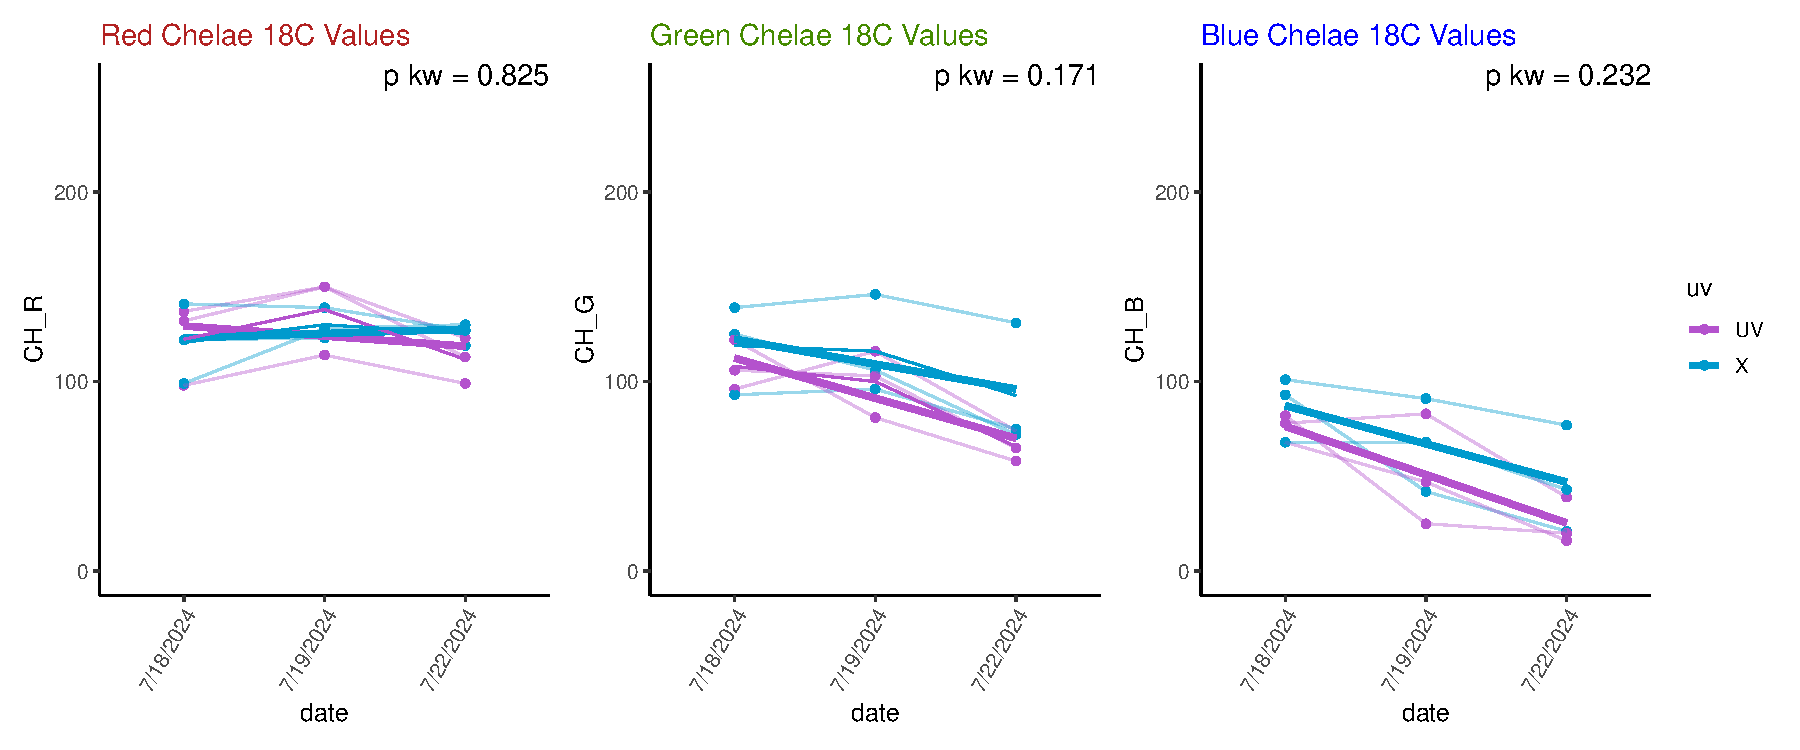
\includegraphics{color_analysis_pdf_files/figure-latex/Line Plots Example-1.pdf}

\end{document}
